\documentclass[journal,12pt,twocolumn]{IEEEtran}

\usepackage{setspace}
\usepackage{gensymb}

\singlespacing


\usepackage[cmex10]{amsmath}

\usepackage{amsthm}

\usepackage{mathrsfs}
\usepackage{txfonts}
\usepackage{stfloats}
\usepackage{bm}
\usepackage{cite}
\usepackage{cases}
\usepackage{subfig}

\usepackage{longtable}
\usepackage{multirow}

\usepackage{enumitem}
\usepackage{mathtools}
\usepackage{steinmetz}
\usepackage{tikz}
\usepackage{circuitikz}
\usepackage{verbatim}
\usepackage{tfrupee}
\usepackage[breaklinks=true]{hyperref}
\usepackage{graphicx}
\usepackage{tkz-euclide}
\usepackage{float}

\usetikzlibrary{calc,math}
\usepackage{listings}
    \usepackage{color}                                            %%
    \usepackage{array}                                            %%
    \usepackage{longtable}                                        %%
    \usepackage{calc}                                             %%
    \usepackage{multirow}                                         %%
    \usepackage{hhline}                                           %%
    \usepackage{ifthen}                                           %%
    \usepackage{lscape}     
\usepackage{multicol}
\usepackage{chngcntr}

\DeclareMathOperator*{\Res}{Res}

\renewcommand\thesection{\arabic{section}}
\renewcommand\thesubsection{\thesection.\arabic{subsection}}
\renewcommand\thesubsubsection{\thesubsection.\arabic{subsubsection}}

\renewcommand\thesectiondis{\arabic{section}}
\renewcommand\thesubsectiondis{\thesectiondis.\arabic{subsection}}
\renewcommand\thesubsubsectiondis{\thesubsectiondis.\arabic{subsubsection}}


\hyphenation{op-tical net-works semi-conduc-tor}
\def\inputGnumericTable{}                                 %%

\lstset{
%language=C,
frame=single, 
breaklines=true,
columns=fullflexible
}
\begin{document}
\newtheorem{theorem}{Theorem}[section]
\newtheorem{problem}{Problem}
\newtheorem{proposition}{Proposition}[section]
\newtheorem{lemma}{Lemma}[section]
\newtheorem{corollary}[theorem]{Corollary}
\newtheorem{example}{Example}[section]
\newtheorem{definition}[problem]{Definition}

\newcommand{\BEQA}{\begin{eqnarray}}
\newcommand{\EEQA}{\end{eqnarray}}
\newcommand{\define}{\stackrel{\triangle}{=}}
\bibliographystyle{IEEEtran}
\providecommand{\mbf}{\mathbf}
\providecommand{\pr}[1]{\ensuremath{\Pr\left(#1\right)}}
\providecommand{\qfunc}[1]{\ensuremath{Q\left(#1\right)}}
\providecommand{\sbrak}[1]{\ensuremath{{}\left[#1\right]}}
\providecommand{\lsbrak}[1]{\ensuremath{{}\left[#1\right.}}
\providecommand{\rsbrak}[1]{\ensuremath{{}\left.#1\right]}}
\providecommand{\brak}[1]{\ensuremath{\left(#1\right)}}
\providecommand{\lbrak}[1]{\ensuremath{\left(#1\right.}}
\providecommand{\rbrak}[1]{\ensuremath{\left.#1\right)}}
\providecommand{\cbrak}[1]{\ensuremath{\left\{#1\right\}}}
\providecommand{\lcbrak}[1]{\ensuremath{\left\{#1\right.}}
\providecommand{\rcbrak}[1]{\ensuremath{\left.#1\right\}}}
\theoremstyle{remark}
\newtheorem{rem}{Remark}
\newcommand{\sgn}{\mathop{\mathrm{sgn}}}
\providecommand{\abs}[1]{\vert#1\vert}
\providecommand{\res}[1]{\Res\displaylimits_{#1}} 
\providecommand{\norm}[1]{\lVert#1\rVert}
%\providecommand{\norm}[1]{\lVert#1\rVert}
\providecommand{\mtx}[1]{\mathbf{#1}}
\providecommand{\mean}[1]{E[ #1 ]}
\providecommand{\fourier}{\overset{\mathcal{F}}{ \rightleftharpoons}}
%\providecommand{\hilbert}{\overset{\mathcal{H}}{ \rightleftharpoons}}
\providecommand{\system}{\overset{\mathcal{H}}{ \longleftrightarrow}}
	%\newcommand{\solution}[2]{\textbf{Solution:}{#1}}
\newcommand{\solution}{\noindent \textbf{Solution: }}
\newcommand{\cosec}{\,\text{cosec}\,}
\providecommand{\dec}[2]{\ensuremath{\overset{#1}{\underset{#2}{\gtrless}}}}
\newcommand{\myvec}[1]{\ensuremath{\begin{pmatrix}#1\end{pmatrix}}}
\newcommand{\mydet}[1]{\ensuremath{\begin{vmatrix}#1\end{vmatrix}}}
\numberwithin{equation}{subsection}
\makeatletter
\@addtoreset{figure}{problem}
\makeatother
\let\StandardTheFigure\thefigure
\let\vec\mathbf
\renewcommand{\thefigure}{\theproblem}
\def\putbox#1#2#3{\makebox[0in][l]{\makebox[#1][l]{}\raisebox{\baselineskip}[0in][0in]{\raisebox{#2}[0in][0in]{#3}}}}
     \def\rightbox#1{\makebox[0in][r]{#1}}
     \def\centbox#1{\makebox[0in]{#1}}
     \def\topbox#1{\raisebox{-\baselineskip}[0in][0in]{#1}}
     \def\midbox#1{\raisebox{-0.5\baselineskip}[0in][0in]{#1}}
\vspace{3cm}
\title{GATE ASSIGNMENT 3}
\author{Amulya Tallamraju \\ AI20BTECH11003}
\maketitle
\newpage
\bigskip
\renewcommand{\thefigure}{\theenumi}
\renewcommand{\thetable}{\theenumi}
Download all python codes from 
\begin{lstlisting}
https://github.com/AmulyaTallamraju/EE3900/blob/main/GATE_Assignment-3/codes/GATE_Assignment-3.py
\end{lstlisting}
%
and latex-tikz codes from 
%
\begin{lstlisting}
https://github.com/AmulyaTallamraju/EE3900/blob/main/GATE_Assignment-3/GATE_Assignment-3.tex
\end{lstlisting}
%
\section{GATE EC 2005 Q.5}
The function $x(t)$ is shown in figure. Even and odd parts of a unit step function u(t) are given by
\begin{figure}[!ht]
         \centering
         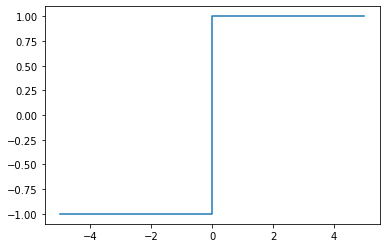
\includegraphics[width=\columnwidth]{question.png}
         \caption{Plot of $x[t]$}
         \label{plot}
\end{figure}
\section{Solution}
\begin{figure}[!ht]
         \centering
         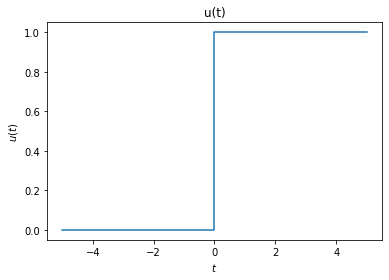
\includegraphics[width=\columnwidth]{u(t).png}
         \caption{Plot of $u[t]$}
         \label{plot}
\end{figure}
\begin{figure}[!ht]
         \centering
         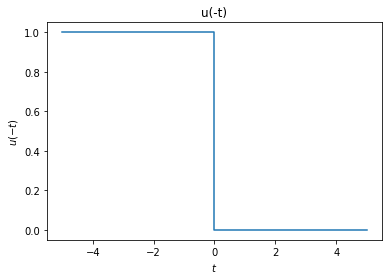
\includegraphics[width=\columnwidth]{u(-t).png}
         \caption{Plot of $u[t]$}
         \label{plot}
\end{figure}
\begin{figure}[!ht]
         \centering
         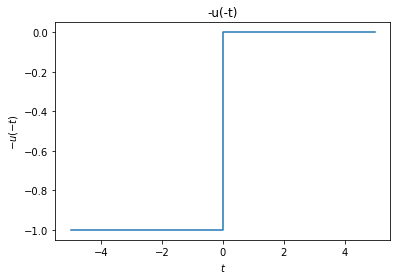
\includegraphics[width=\columnwidth]{-u(-t).png}
         \caption{Plot of $-u[-t]$}
         \label{plot}
\end{figure}
\begin{align} x(t)=\begin{cases} 
      -1 & x\leq 0 \\
      0 & 0\leq x=0 \\
      1 & x\geq 0
   \end{cases}
\end{align}
From the above definition of $x(t)$ we can see that it is the same as $sgn(t)$.
Odd part of $u(t)$ is given by
\begin{align}
    \frac{u(t)-u(-t)}{2}
\end{align}
One observing the plots of $x(t),u(t),-u(-t)$ we can see that
\begin{align}
    x(t)=u(t)-u(-t)
\end{align}
Thus, the odd part of $u(t)$ is $\frac{x(t)}{2}$.
The even part of u(t) is given by
\begin{align}
 \frac{u(t)+u(-t)}{2} &=\frac{1}{2}  
\end{align}
Thus the even and odd parts of the unit step signal are
\begin{align}
   \frac{1}{2} , \frac{x(t)}{2}
\end{align}
The fourier transform of $x(t)$ is given by
\begin{align}
     \mathcal{F} \{x(t)\}= \int_{ - \infty }^{ + \infty } x(t){e^{ - j\omega t}}dt
\end{align}
This signal is not absolutely integrable so we calculate Fourier Transform of $x(t)$ as a limiting case of the sum of exponential $e^{-at}u(t) - e^{at}u(t)$ as $a \to 0.$
\begin{align}
    \mathcal{F} \{x(t)\}&=\lim_{a \to 0} \int_{ - \infty }^{ + \infty } \brak{e^{-at}u(t) - e^{at}u(t)}{e^{ - 2\pi fj t}}dt\\
    &=\lim_{a \to 0}\sbrak{\frac{1}{a  +  2\pi fj}  -  \frac{1}{a  - 2\pi f j}}\\
    &=\frac{1}{\pi f j}
\end{align}
The fourier transform of the unit step function can be found by realising that
\begin{align}
u(t)=\frac12(1+\sgn(t))    
\end{align}
\begin{align}
 \implies   \mathcal{F}\{u(t)\}&=\frac12\left(\mathcal{F}\{1\}+\mathcal{F}\{\text{sgn}(t)\}\right)\\&=\pi\delta(f)+\frac{1}{2\pi fj}
\end{align}
The Double-sided Laplace transform of $x(t)$
\begin{align}
    \mathcal{L}\{x\}(s) &= \int_{-\infty}^{\infty} x(t)e^{-st} \, dt.\\
    &=\frac{2}{s}
\end{align}
\end{document}
